% -------------------------允许算法跨页-------------
\makeatletter
\newenvironment{breakablealgorithm}
{% \begin{breakablealgorithm}
	\begin{center}
		\refstepcounter{algorithm}% New algorithm
		\hrule height.8pt depth0pt \kern2pt% \@fs@pre for \@fs@ruled
		\renewcommand{\caption}[2][\relax]{% Make a new \caption
			{\raggedright\textbf{\ALG@name~\thealgorithm} ##2\par}%
			\ifx\relax##1\relax % #1 is \relax
			\addcontentsline{loa}{algorithm}{\protect\numberline{\thealgorithm}##2}%
			\else % #1 is not \relax
			\addcontentsline{loa}{algorithm}{\protect\numberline{\thealgorithm}##1}%
			\fi
			\kern2pt\hrule\kern2pt
		}
	}{% \end{breakablealgorithm}
		\kern2pt\hrule\relax% \@fs@post for \@fs@ruled
	\end{center}
}
\makeatother

%----------------------------------------------------
\documentclass[11pt,a4paper]{ctexart}
\usepackage{fontspec}
\usepackage{xeCJK}%文字体的设置
%\newcommand{\canger}{\CJKfontspec{TsangerJinKai03}}
%\setmainfont{TsangerJinKai03} %设置全文字体
%\setsansfont{TsangerJinKai03}
%\setsansfont{TsangerJinKai03} 
%\defaultfontfeatures{Mapping=tex-text}
%\setCJKmainfont{TsangerJinKai03}
%\setCJKsansfont{TsangerJinKai03}
\usepackage{xunicode}
\usepackage{xltxtra}
\usepackage{amsmath}
\usepackage{amsfonts}
\usepackage{amssymb}
\usepackage{graphicx}
\usepackage{amsthm}
\usepackage{array}
\usepackage{tcolorbox}
\usepackage{float}   %{H}
\usepackage{booktabs}  %\toprule[1.5pt]
\usepackage[titletoc]{appendix}
\usepackage{algorithm}  
\usepackage{algorithmic}  
%\usepackage{algorithmicx}
%===================%插入代码需要的控制
\usepackage{listings}
\usepackage{xcolor}
\setmonofont{Consolas}%字体
\lstset{%
	numbers=left,
	numberstyle=\tt\tiny,%
	showstringspaces=false,
	showspaces=false,%
	tabsize=4,%
	frame=lines,%
	basicstyle=\tt\small,%
	keywordstyle=\color{ blue!70}\bfseries,%
	identifierstyle=,%
	commentstyle=\color{red!50!green!50!blue!50},%\itshape,%
	stringstyle=\color{black},%
	breaklines=true
}
%===================%
\usepackage[left=2cm,right=2cm,top=2cm,bottom=2cm]{geometry}
\newtheorem*{solution}{解}
\newtheorem{cor}{推论}
\newtheorem{e}{习题}
\title{算法设计与分析(5.20作业)}
\author{智科三班 \quad 严中圣 \quad 222020335220177}
\date{\today}
\begin{document}
\maketitle
\pagestyle{plain}%设置页码
%\noindent\rule{\textwidth}{1pt} %加横线
%============================================================================

\begin{tcolorbox}[colback=white!10!white,colframe=pink!100!black]
	\begin{figure}[H]
		\centering
		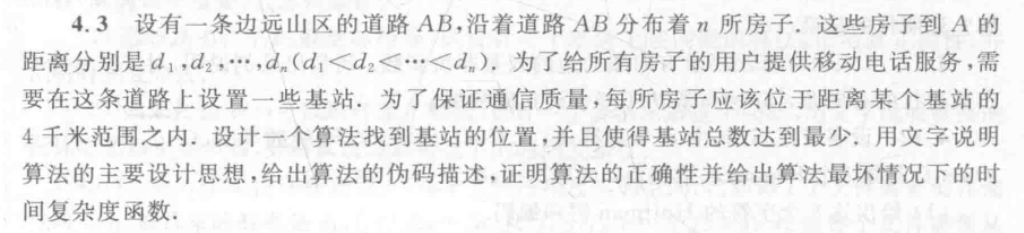
\includegraphics[width=0.8\linewidth]{screenshot033}
		%\caption{}
		\label{fig:screenshot033}
	\end{figure}
\end{tcolorbox}
\begin{solution}
\end{solution}
为了使基站总数达到最少,就要求要最大化地利用每个基站,即让每个基站的辐射范围内尽可能多地覆盖住宅。利用贪心算法,从第一个住宅后4km的位置开始扫描,以扫描中心点附近4km内的住宅为标准,搜索到最大覆盖住宅数即在此处放置基站,直道所有住宅均被覆盖后停止搜索,算法结束。如此便可得到最少基站总数。

伪码描述如下:
\begin{breakablealgorithm}
	\caption{4.3 } 
	\begin{algorithmic}[1]
		\REQUIRE $D[n]$ //距离数据,$D[i]$表示住宅$i$到$A$的距离,$i=1,2,...,n$,为了简便,假设每个元素值均为整数,单位为km
		\ENSURE 最小基站总数
		\STATE $Initialize$ $S$ //基站位置
		\STATE $count \gets$ 1
		\STATE $S[count]=D[1]+4$
		\FOR {$j \gets 2 \; \textbf{to} \; n$}
				\IF {$D[j]-S[count]<4$}
					\STATE $count\gets count+1$
					\STATE $S[count]=D[j]+4$
				\ENDIF
		\ENDFOR
		\RETURN $count$
	\end{algorithmic}
\end{breakablealgorithm}
下面对算法的正确性进行证明,即需要证明对前$k(k\in N)$步操作,存在最优方案包含前$k$步选择的基站。对步数归纳进行证明:
\begin{enumerate}
	\item[(1)]
	当$k=1$时,必定存在最优策略包含$S[1]$。如果不包含,假设最优解第一个基站位置为$T[1]$,则$T[1]$必定小于$S[1]$,否则无法覆盖到第一个住宅,所以$T[1]$的辐射范围的住宅均在$S[1]$的覆盖范围内,所以用$S[1]$替换$T[1]$仍然是最优解。
	\item[(2)]
	假设第$k$步时,存在最优策略包含前$k$步选择的基站,即包含了$\{S[1],S[2],...,S[k]\}$,假设前k个基站覆盖了$d_1,d_2,...,d_m$,最优解剩余基站$\{T[k+1],T[k+2]...\}$覆盖了$d_{m+1},...d_n$。
	
	当第$k+1$步时,假设$T[k+1]$覆盖了$d_{m+1},...,d_{m+j}$,与$k=1$时类似,此时$T[k+1]\leq S[k+1]$,故用$S[k+1]$替代后仍然为最优解,所以第$k+1$步时存在最优解包含前$k+1$步选择的基站。证毕。
\end{enumerate}
算法的时间复杂度为$O(n)$。
\begin{tcolorbox}[colback=white!10!white,colframe=pink!100!black]
\begin{figure}[H]
	\centering
	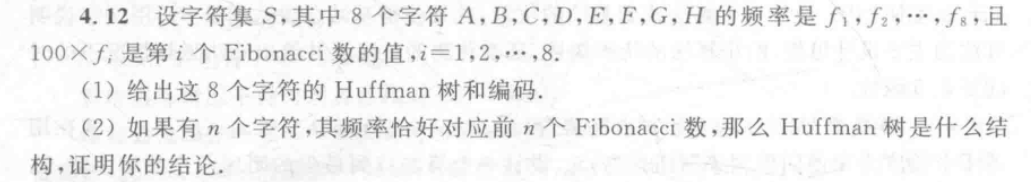
\includegraphics[width=0.9\linewidth]{screenshot034}
	%\caption{}
	\label{fig:screenshot034}
\end{figure}
\end{tcolorbox}
\begin{solution}
\end{solution}
(1)易得$f_1=100,f_2=100,f_3=200,f_4=300,f_5=500,f_6=800,f_7=1300,f_8=2100$

Huffman树及编码如下:
\begin{figure}[H]
	\centering
	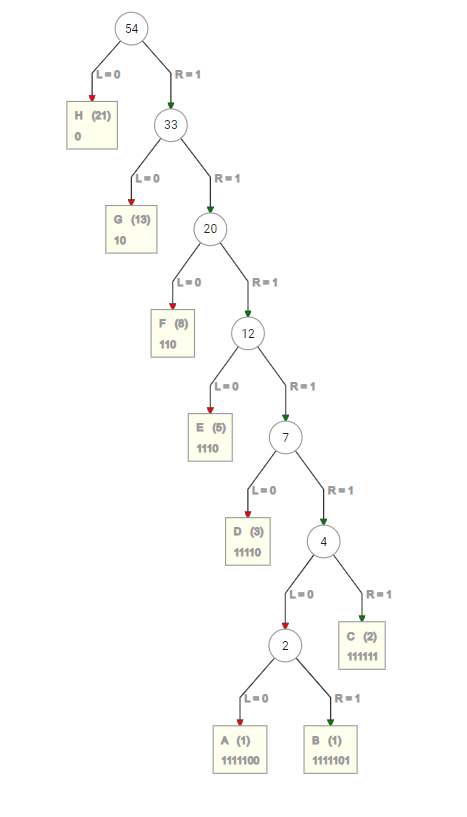
\includegraphics[width=0.5\linewidth]{screenshot036}
	%\caption{}
	\label{fig:screenshot036}
\end{figure}

(2)由于Fibonacci数列从第三项开始即单调递增,同时可以发现对第$k(k\geq3)$项,
\begin{gather}
	F(k+1) < \sum_{i=1}^{k}F(i) < F(k+2) 
\end{gather}
故在构造Huffman树时,从第三项开始,Huffman均为单链式结构。下面对式(1)进行证明。
\begin{enumerate}
	\item[(1)]当$k=3$时,$F(4)=3<\sum_{i=1}^{3}=4<F(5)=5$,满足条件。
	\item[(2)]假设当$k=n(n\in N ,n\geq 3)$时,$F(n+1) < \sum_{i=1}^{n}F(i) < F(n+2) $;
	
	当$k=n+1$时,$\because F(n+2)=F(n+1)+F(n) ,\therefore F(n+2)-F(n+1)<\sum_{i=1}^{n}F(i),$即$F(n+2)<\sum_{i=1}^{n+1}F(i)$,等式左半边得证;
	
	又$\because F(n+3)=F(n+2)+F(n+1),\therefore\sum_{i=1}^{n}F(i)+F(n+1)<F(n+2)+F(n+1)$,即$\sum_{i=1}^{n+1}F(i)<F(n+3)$,至此证毕。
\end{enumerate}

%相应伪码如下:
%\begin{breakablealgorithm}
%	\caption{3.3 库房出租问题} 
%	\begin{algorithmic}[1]
%		\REQUIRE $D,L,V$ \quad 库房总长度限制,货柜长度数据,货柜收益数据
%		\ENSURE 最大收益以及货柜选择
%		\STATE $Initialize$ $M[n][D]$//dp矩阵,初始化为0
%		\STATE $Initialize$ $S[n][D]$//结果矩阵,存储最优解方案下的货柜选择
%		\FOR {$j\gets 1 \; \textbf{to} \; D$}
%			\STATE $M[1,j]\gets V[1]$
%		\ENDFOR
%		\FOR {$i\gets 2 \;\textbf{to} \; n$}
%			\FOR {$j\gets 1 \;\textbf{to} \; D$}
%				\IF {$L_i \leq j$}
%					\IF {$M[i-1][j]<M[i-1][j-l_i]+v_i$}
%						\STATE $M[i][j] = M[i-1][j-l_i]+v_i$
%						\STATE $S[i][j]=i$
%					\ELSE
%						\STATE $M[i][j] =M[i-1][j]$
%						\STATE $S[i][j]=S[i-1][j]$
%					\ENDIF
%				\ELSE
%					\STATE $M[i][j] =M[i-1][j]$
%					\STATE $S[i][j]=S[i-1][j]$
%				\ENDIF
%			\ENDFOR
%		\ENDFOR
%		\RETURN $M[n][D]$
%	\end{algorithmic}
%\end{breakablealgorithm}
%算法最坏情况下的时间复杂度为$O(nD)$。
%
%\begin{tcolorbox}[colback=white!10!white,colframe=pink!100!black]
%	\begin{figure}[H]
%		\centering
%		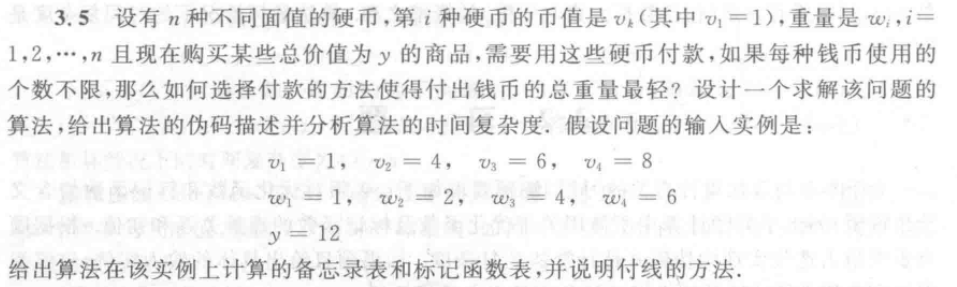
\includegraphics[width=0.8\linewidth]{screenshot019}
%		\label{fig:screenshot019}
%	\end{figure}
%\end{tcolorbox}
%\begin{solution}
%\end{solution}
%根据题意定义$x_i$为第$i$种硬币使用的个数,$x_i$为非负整数,则目标函数为
%\begin{equation*}
%	W = \min \sum_{i=1}^{n}\omega_ix_i\quad ,\sum_{i=1}^{n}v_ix_i=y
%\end{equation*}
%设定dp矩阵$W[n][y]$,$W[i][j]$表示使用前$i$种硬币,总价值为$j$时的最优解重量。结果矩阵$S[n][y]$,$S[i][j]$表示最优解时选择的硬币的最大标号。
%递推方程如下:
%\begin{gather*}
%	W[i][j] = \min\{W[i-1][j],W[i][j-v_i]+\omega
%	_i\} \quad,i>1,0<j\leq y \\
%	W[1][j] = \omega_1 j  \quad,0<j\leq q\\
%	W[i][0] = 0 \quad,0<i\leq n \\ 
%	W[i][j] = +\infty \quad,j<0 \\
%	S[i][j] = \left\{
%	\begin{aligned}
%		&i \quad ,W[i-1][j]\geq W[i][j-v_i]+\omega_i \\
%		&S[i-1][j]\quad ,else \\
%	\end{aligned}
%	\quad,i>1,0<j\leq y
%	\right. \\
%	S[1][j] = 1 \quad,0<j\leq y \\
%	S[i][0] = 0 \quad,1\leq i \leq n \\
%\end{gather*}
%由上伪码如下:
%\begin{breakablealgorithm}
%	\caption{3.5 硬币选择问题} 
%	\begin{algorithmic}[1]
%		\REQUIRE $\omega,V,y$ \quad $\omega$为不同面值硬币的重量,$V$不同面值的硬币,$y$为付款数
%		\ENSURE 总重量最轻的付款的方法
%		\STATE $initialize \quad W[n][y] $ //dp数组
%		\STATE $initialize \quad  S[n][y] $ //结果数组
%		\FOR {$j\gets 1 \; \textbf{to} \; y$}
%			\STATE $W[1][j]\gets \omega_1 j$
%			\STATE $S[1][j] \gets 1$
%		\ENDFOR
%		\FOR {$i\gets 2 \; \textbf{to} \; n$}
%			\FOR {$j\gets 1 \; \textbf{to} \; y$}
%				\IF {$W[i-1][j]\geq W[i][j-v_i]+\omega_i$}
%					\STATE $W[i][j] = W[i][j-v_i]+\omega_i$
%					\STATE $S[i][j]=i$
%				\ELSE
%					\STATE $W[i][j] =W[i-1][j]$
%					\STATE $S[i][j]=S[i-1][j]$
%				\ENDIF
%			\ENDFOR
%		\ENDFOR
%		\RETURN $W[n][y]$
%	\end{algorithmic}
%\end{breakablealgorithm}
%将实例代入上述解法代码求解(附录2)得备忘录和结果矩阵如下所示:
%\begin{figure}[H]
%	\centering
%	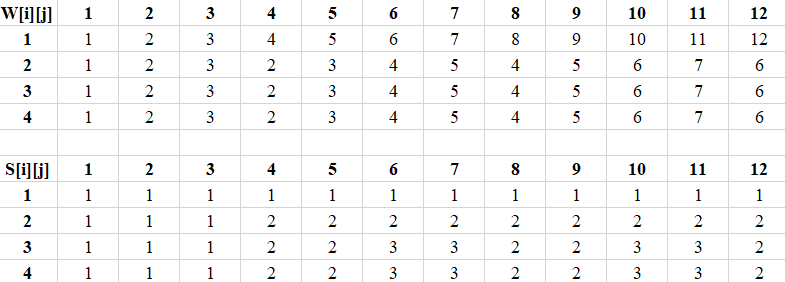
\includegraphics[width=0.7\linewidth]{screenshot032}
%	\caption{}
%	\label{fig:screenshot032}
%\end{figure}
%
%由此可得,最轻重量为$W[4][12]=6$,$S[4][12]=2$,所以$x_3=x_4=0,x_2\geq 1$,$S[2][8]=2,S[2][4]=2,S[2][0]=0$,所以$x_2=3,x_1=0$。
%故最终解为,$x_1=0,x_2=3,x_3=0,x_4=0$,最轻重量为6.
%\newpage
%\huge{\centering \textbf{附录1}}
%\begin{lstlisting}[language=c++]
%	#include <iostream>
%	#include <cmath>
%	#include <cstring>
%	#include <vector>
%	using namespace std;
%	int main()
%	{
%		int F[3][11];
%		int S[3][11];
%		int G[3][4] = {{2, 4, 7, 11}, {5, 10, 16, 20}, {8, 12, 17, 22}};
%		memset(F, 0, sizeof(F));
%		memset(S, 0, sizeof(S));
%		for (int i = 0; i < 11; i++)
%		{
%			F[0][i] = G[0][(int)sqrt(i)];
%		}
%		for (int i = 1; i < 3; ++i)
%		{
%			for (int j = 0; j < 11; j++)
%			{
%				int max = 0;
%				int index = 0;
%				for (int k = 0; k <= (int)sqrt(j); k++)
%				{
%					if (F[i - 1][j - k * k] + G[i][k] > max)
%					{
%						max = F[i - 1][j - k * k] + G[i][k];
%						index = k;
%					}
%				}
%				F[i][j] = max;
%				S[i][j] = index;
%			}
%		}
%		for (int i = 0; i < 3; i++)
%		{
%			for (int j = 0; j < 11; j++)
%			{
%				cout << F[i][j] << " ";
%			}
%			cout << endl;
%		}
%		for (int i = 0; i < 3; i++)
%		{
%			for (int j = 0; j < 11; j++)
%			{
%				cout << S[i][j] << " ";
%			}
%			cout << endl;
%		}
%		return 0;
%	}
%\end{lstlisting}
%
%\huge{\centering \textbf{附录2}}
%\begin{lstlisting}[language=c++]
%	#include <iostream>
%	#include <cstring>
%	using namespace std;
%	int main()
%	{
%		int W[4][13];
%		int S[4][13];
%		int V[4] = {1, 4, 6, 8};
%		int w[4] = {1, 2, 4, 6};
%		memset(W, 0, sizeof(W));
%		memset(S, 0, sizeof(S));
%		for (int j = 1; j <= 12; j++)
%		{
%			W[0][j] = j * w[0];
%			S[0][j] = 1;
%		}
%		for (int i = 1; i < 4; ++i)
%		{
%			for (int j = 1; j <= 12; j++)
%			{
%				if (W[i - 1][j] >= (W[i][j - V[i]] + w[i]))
%				{
%					W[i][j] = W[i][j - V[i]] + w[i];
%					S[i][j] = i + 1;
%				}
%				else
%				{
%					W[i][j] = W[i - 1][j];
%					S[i][j] = S[i - 1][j];
%				}
%			}
%		}
%		for (int i = 0; i < 4; i++)
%		{
%			for (int j = 1; j <= 12; j++)
%			{
%				cout << W[i][j] << " ";
%			}
%			cout << endl;
%		}
%		for (int i = 0; i < 4; i++)
%		{
%			for (int j = 1; j <= 12; j++)
%			{
%				cout << S[i][j] << " ";
%			}
%			cout << endl;
%		}
%	}
%\end{lstlisting}
%\begin{tcolorbox}[colback=white!10!white,colframe=pink!100!black]
%	\begin{figure}[H]
%		\centering
%		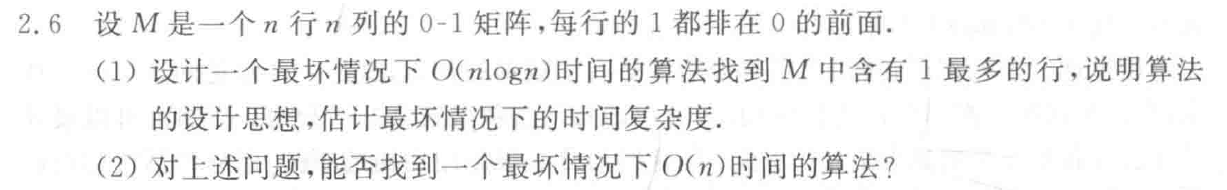
\includegraphics[width=0.9\linewidth]{screenshot017}
%		\label{fig:screenshot017}
%	\end{figure}
%\end{tcolorbox}
%\begin{solution}
%\end{solution}
%(2)对于$O(n)$的算法设计如下:从第一行开始查找至最后一个为1的位置,记录此时的列号,向下寻找,若寻找到某一行该位置也为1,则在该行继续向后查找至最后一个为1的位置,重复该操作直至走到矩阵最下方。伪码如下:
%\begin{breakablealgorithm}
%	\caption{2.6 \quad $O(n)$算法}
%	\begin{algorithmic}[1]
%		\REQUIRE $M$ \quad 题设矩阵,假设每一行1的个数都不相等
%		\ENSURE $TargetRow$ \quad $M$种含有1最多的行
%		\STATE $TargetRow\gets 1,column\gets 1,row\gets 1$
%		\WHILE {$row \leq n$}
%			\IF {$M[row][column] == 0$}
%				\STATE $row \gets row+1$
%			\ELSE
%				\STATE $TargetRow \gets row$
%				\FOR {$i\gets column \;\textbf{to}\;n$}
%					\IF {$M[row][i] == 1$}
%						\STATE $column \gets i$
%					\ELSE
%					 	\STATE $\textbf{break}$
%					\ENDIF
%				\ENDFOR
%				\STATE $row \gets row+1$
%			\ENDIF
%		\ENDWHILE
%		\RETURN $TargetRow$
%	\end{algorithmic}
%\end{breakablealgorithm}

%\begin{tcolorbox}[colback=white!10!white,colframe=pink!100!black]
%	\begin{figure}[H]
%		\centering
%		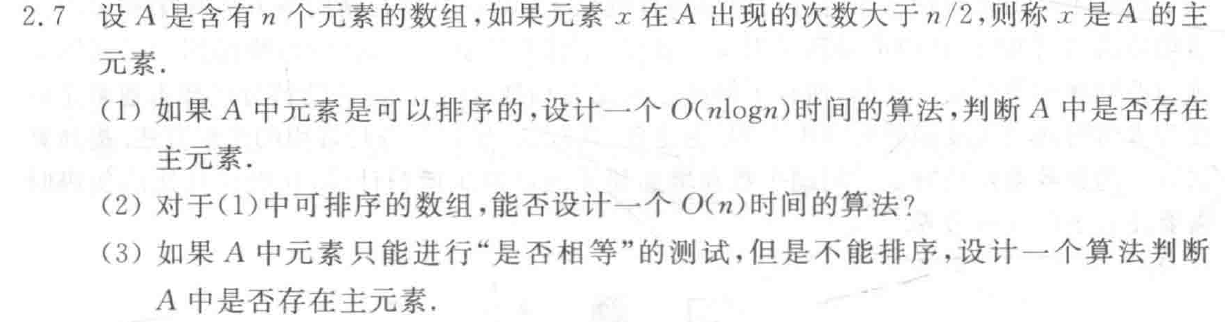
\includegraphics[width=0.9\linewidth]{screenshot018}
%		\label{fig:screenshot018}
%	\end{figure}
%\end{tcolorbox}
%\begin{solution}
%\end{solution}
%(2)利用$O(n)$的排序算法,排序后再进行顺序查找,对相同元素计数,总时间复杂度为$O(n)+O(n)=O(n)$,伪代码如下所示:
%\begin{breakablealgorithm}
%	\caption{2.7 \qquad $O(n)$算法}
%	\begin{algorithmic}[1]
%		\REQUIRE $A$ \quad 题设数组
%		\ENSURE $STATUS$ \quad 布尔量,若存在主元素则为$True$
%		\STATE $STATUS \gets True$
%		\STATE $A \gets sort(A)$ //利用$O(n)的排序算法进行排序$
%		\STATE $count \gets 0,number \gets A[1],n\gets \vert A \vert$
%		\FOR {$i\gets 1 \;\textbf{to}\; n$}
%			\IF {$A[i] == number$}
%				\STATE $count \gets count+1$
%				\IF {$count > \frac{n}{2}$}
%					\RETURN $True$
%				\ENDIF
%			\ELSE
%				\STATE $number \gets A[i]$
%				\STATE $count \gets 1$
%			\ENDIF
%		\ENDFOR
%		\RETURN $False$
%	\end{algorithmic}
%\end{breakablealgorithm}
%(3)
%直接利用暴力算法即直接让每一个数和数组中每个元素进行相等测试,则可得到每个数出现的次数,再与$n/2$比较即可得出结果,该算法时间复杂度显然是$O(n^2)$的。伪码如下所示:
%\begin{breakablealgorithm}
%	\caption{2.7(3) \qquad 暴力算法}
%	\begin{algorithmic}[1]
%		\REQUIRE $A$ \quad 题设数组
%		\ENSURE $STATUS$ \quad 布尔量,若存在主元素则为$True$
%		\STATE $STATUS \gets True$
%		\STATE $n\gets \vert A \vert$
%		\FOR {$i\gets 1 \;\textbf{to}\; \frac{n+1}{2}$}
%			\STATE $number \gets A[i],count \gets 0$
%			\FOR {$j \gets 1 \; \textbf{to}\; n$}
%				\IF {$A[i] == number$}
%					\STATE $count \gets count+1$
%				\ENDIF
%				\IF {$count > \frac{n}{2}$}
%					\RETURN $True$
%				\ENDIF
%			\ENDFOR
%		\ENDFOR
%		\RETURN $False$
%	\end{algorithmic}
%\end{breakablealgorithm}

\end{document}